\documentclass[a4paper,12pt]{article}
\usepackage{mathrsfs}
\usepackage[utf8]{inputenc}
\usepackage[spanish]{babel}
\usepackage{amsmath}
\usepackage{amsfonts}
\usepackage{amssymb} 
\usepackage{graphicx} 
\usepackage{hyperref} 
\usepackage{wrapfig}
\usepackage{enumitem}
\usepackage{fancyhdr}
\usepackage{float}
\usepackage{eurosym}
\usepackage{color}
\usepackage{circuitikz}
\usepackage{titling}
\usepackage{hyperref}
\usepackage{media9}
\usepackage{lipsum}
\usepackage{tocbibind}
\usepackage{listings}
\usepackage{tabularx}
\usepackage{tcolorbox}
\usepackage{bookmark}
\usepackage{media9}
\usepackage[table]{xcolor}
\definecolor{lightblue}{RGB}{228, 244, 253}
\usepackage{listings}
\usepackage{color}

\definecolor{dkgreen}{rgb}{0,0.6,0}
\definecolor{gray}{rgb}{0.5,0.5,0.5}
\definecolor{mauve}{rgb}{0.58,0,0.82}

\lstset{frame=tb,
  language=Python,
  inputencoding=utf8,
  extendedchars=true,
  aboveskip=3mm,
  belowskip=3mm,
  showstringspaces=false,
  columns=flexible,
  basicstyle={\small\ttfamily},
  numbers=none,
  numberstyle=\tiny\color{gray},
  keywordstyle=\color{blue},
  commentstyle=\color{dkgreen},
  stringstyle=\color{mauve},
  breaklines=true,
  breakatwhitespace=true,
  tabsize=3,
  literate=%
    {á}{{\'a}}1
    {é}{{\'e}}1
    {í}{{\'i}}1
    {ó}{{\'o}}1
    {ú}{{\'u}}1
    {ñ}{{\~n}}1
    {č}{{\v{c}}}1
}
\usepackage[left=3cm,right=3cm,top=3cm,bottom=4cm]{geometry}
\sloppy

\pagestyle{fancy}
\providecommand{\abs}[1]{\lvert#1\rvert}
\providecommand{\norm}[1]{\lVert#1\rVert}

%%% Para las cabeceras
\newcommand{\hsp}{\hspace{20pt}}
\newcommand{\HRule}{\rule{\linewidth}{0.5mm}}
\headheight=50pt
%%% 
\newcommand{\vacio}{\textcolor{white}{ .}}

%%% Para que las ecuaciones se numeren
%%% con el número de sección y el de ecuación.
\renewcommand{\theequation}{\thesection.\arabic{equation}}


% Color azul para algunos 
% textos de la portada
\definecolor{azulportada}{rgb}{0.16, 0.32, 0.75}

%%%% Azul para textos de headings
\definecolor{azulinterior}{rgb}{0.0, 0.2, 0.6}

%%%%%%%%%%%%%%%%%%%%%%%%%%%%%%%%
%%%%%% Datos del proyecto %%%%%%
%%%%%%%%%%%%%%%%%%%%%%%%%%%%%%%%
%%%TÍTULO
%%% Escribirlo en minúsculas, el programa
%%% lo pondrá en mayúsculas en la portada.

\title{Procesamiento de imágenes}

%%%% AUTORES
\author{Lydia Ruiz Martínez \and Pablo Tuñón Laguna}

%%%%%%%%%%%%%%%%%%%%%
%%%%%%%%%%%%%%%%%%%%
\begin{document}

%%%%%%%%%%%%%%%%%%%%%%%%%%%%%%%
%%%%%%%%%%%%%%%%%%%%%%%%%%%%%%%
\begin{titlepage} %%%%% Aquí no hay que tocar nada.
	%%%% Las siguientes instrucciones generarán automáticamente
	%%%% la portada de tu proyecto.
	%%% Cambio de la estructura de esta página
\newgeometry{left=0.6cm,top=1.3cm,bottom=1.2cm}

\fbox{\parbox[c]{18.5cm}{
\begin{center}
\vspace{1.5cm}
{\fontfamily{ptm}\fontsize{24}{28.8}\selectfont{Universidad Pontificia de Comillas}}\\
[3.5em]
{\fontfamily{ptm}\fontsize{24}{5}\selectfont{ICAI}}\\
[4.5em]
{\fontfamily{ptm}\fontsize{28}{5}\selectfont{LABORATORIO 2}}\\
[2cm]
{\fontfamily{ptm}\fontsize{24}{5}\selectfont{Visión por Ordenador I}}\\
[2cm]

% Autor del trabajo de investigación
\textcolor{azulportada}{\fontfamily{ptm}\fontsize{16}{5}\selectfont{\theauthor}}\\
[2cm]
% Título del trabajo
\textcolor{azulportada}
{\fontfamily{ptm}\fontsize{30}{5}\selectfont{\textsc{\thetitle}}}\\
%{\Huge\textbf{\thetitle}}\\
[1.2cm]

\includegraphics[width=10cm]{fonts/Logo ICAI.png}
\\[1.8cm]

{\fontfamily{ptm}\fontsize{16}{5}\selectfont{Curso 2024-2025}}\\
[4cm]
\end{center}
}}
\end{titlepage}
 
 \restoregeometry
 %%%% Volvemos a la estructura de la página normal

%%%%%%%%%%%%%%%%%%%%%%%%%%%%%%

{%\Large

%%%Encabezamiento y pie de página
%%% También se genera automáticamente
%%% Mejor no tocarlo mucho.
\renewcommand{\headrulewidth}{0.5pt}
\fancyhead[R]{
\textcolor{azulportada}{\fontfamily{ptm}\fontsize{10}{3}\selectfont{Laboratorio 2 de Visión por Ordenador I}}\\
{\fontfamily{ptm}\fontsize{10}{3}\selectfont{\theauthor}}}
\fancyhead[L]{
  \textcolor{azulinterior}{\fontfamily{ptm}\fontsize{14}{4}\selectfont{\textbf{\thetitle}}}\\
}

\pagestyle{fancy}
\renewcommand{\footrulewidth}{0.5pt}
\fancyfoot[L]{\footnotesize Universidad Pontificia de Comillas (ICAI) --- curso 2024-2025}
\fancyfoot[C]{\vacio}
\fancyfoot[R]{\footnotesize Página \thepage}

%%%%%%%%%%%%%%%%%%%%
\newpage

\renewcommand{\contentsname}{Índice}
\addtocontents{toc}{\protect\setcounter{tocdepth}{-1}} % Quita el índice de la tabla de contenidos
\tableofcontents
\addtocontents{toc}{\protect\setcounter{tocdepth}{2}}

\newpage


\section{Introducción}


\vspace{1cm}

El procesamiento de imágenes es un área fundamental de la visión por ordenador, esta se enfoca en la manipulación y el análisis
de imágenes digitales. A diferencia de un ser humano, que puede interpretar imágenes de manera intuitiva, un ordenador necesita
algoritmos específicos que le permitan extraer información útil de las matrices de píxeles que componen cada imagen. Estos 
algoritmos permiten a los sistemas de visión por ordenador realizar tareas como la segmentación, la detección de bordes 
y la aplicación de filtros, convirtiendo datos visuales en información comprensible.

\vspace{0.5cm}

La segmentación de imágenes por color es una técnica crucial que permite identificar y aislar objetos de interés en una imagen 
basándose en sus características cromáticas. Este proceso es esencial en múltiples aplicaciones, desde la automatización 
industrial hasta la medicina, donde la identificación precisa de regiones de interés puede marcar la diferencia en el análisis
y la toma de decisiones. La capacidad de un ordenador para diferenciar colores y reconocer patrones en el espacio de color 
adecuado es un paso inicial vital en la interpretación de las imágenes.

\vspace{0.5cm}
La aplicación de filtros es otra herramienta relevante en el procesamiento de imágenes. Filtros como el gaussiano, el de
Sobel o el de Canny se utilizan para suavizar imágenes, eliminar el ruido y detectar bordes, respectivamente. La detección de bordes
es especialmente relevante, ya que resalta las transiciones significativas en una imagen, facilitando la identificación de 
 formas y estructuras. Al aplicar y comparar estos filtros, se puede evaluar tanto la variación en la calidad de la imagen como
la eficiencia en la detección de bordes.

\vspace{0.5cm}
Finalmente, el uso de operadores morfológicos complementa estas técnicas al permitir la manipulación de la estructura de componentes
de una imagen píxel a píxel. Se trata de un enfoque fundamental para mejorar los resultados de la segmentación y la 
detección que además permite desarrollar una comprensión más profunda de las características presentes en las imágenes. En el siguiente estudio, 
se llevarán a cabo implementaciones de las técnicas mencionadas a través de las librerías de Python OpenCv, Imageio y Numpy con el objetivo de
desarrollar un conocimiento práctico de las herramientas de procesamiento de imágenes y su aplicación en la visión por ordenador.

\newpage


\section{Segmentación}


\vspace{1cm}

La segmentación de imágenes por colores es una técnica sencilla y útil en aplicaciones en las que se tiene un gran control
sobre las condiciones de contorno: iluminación, tipo de objeto que se espera encontrar, color de fondo, etc.
En un primer momento se realizaron pruebas de segmentación de imágenes con los colores naranja y blanco, sin embargo, posteriormente
se realizó una adaptación que permite al usuario segmentar cualquier color de su elección.

\vspace{0.5cm}

\subsection{Carga de imágenes}

\vspace{0.5cm}

Todo proceso de visión por ordenador comienza con la carga de las imágenes a procesar, sin embargo hay múltiples formas de llevar 
a cabo este proceso. En el caso de la segmentación de imágenes por color este paso es especialmente importante. Para cargar las imágenes
a partir de su ruta de almacenamiento (obtenida a través de \textit{glob.glob()}) se pueden usar dos procesos análogos:

\vspace{0.5cm}

\begin{itemize}
  \item \textit{cv2.imread()}: La función de la librería \textit{cv2} carga las imágenes en formato RGB.

  \item \textit{imageio.imread()}: La función de la librería \textit{imageio} carga las imágenes en formato BGR.
\end{itemize}

\vspace{0.5cm}

Esta transformación de formato es relevante ya que si se diseña un algoritmo de segmentación de colores en un espacio, no funcionará 
si recibe otro espacio de color ya que los canales de color se interpretan de manera diferente. Esto se puede observar al cargar 
la misma imagen sin realizar ninguna transformación y visualizarla en ambos formatos:

\vspace{0.5cm}

\begin{figure}[H]
  \centering
  \begin{minipage}[t]{0.35\textwidth}
      \centering
      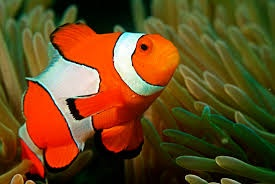
\includegraphics[width=\textwidth]{processed_data/cv2_charged_0.jpg} 
      \caption{Imagen 1 cargada con \textit{cv2.imread()}, formato RGB, autoría propia.}
      \label{fig:cv2_charged}
  \end{minipage}
  \hfill
  \begin{minipage}[t]{0.35\textwidth}
      \centering
      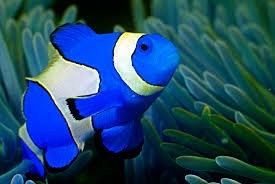
\includegraphics[width=\textwidth]{processed_data/imageio_charged_0.jpg}
      \caption{Imagen 1 cargada con \textit{imageio.imread()}, formato RGB, autoría propia.}
      \label{fig:imageio_charged}
  \end{minipage}
\end{figure}

\subsection{Segmentación monocolor}

\vspace{0.5cm}

Cargadas ya las imágenes se procede a transformarlas al espacio de color HSV ya que genera un mayor contraste : Hue (brillo), Saturation (saturación) y Value (valor).
Para ello se usa la función \textit{cv2.cvtColor()} de OpenCV, que recibe como argumentos la imagen y el espacio de color al que se desea transformar. Una vez que las 
imágenes estén en el espacio de color adecuado, se procede a generar máscaras necesarias, que permiten segmentar los colores de interés. A continuación se muestran los
valores de los umbrales HSV para las imágenes de naranja y blanco:

\vspace{0.5cm}

{\centering
$\text{Naranja}_{min}$; H: 1, S: 190, V: 200 \\
$\text{Naranja}_{max}$; H: 255, S: 255, V: 255 \\
$\text{Blanco}_{min}$; H: 0, S: 0, V: 150 \\
$\text{Blanco}_{max}$; H: 255, S: 50, V: 255\\}

\vspace{0.5cm}

Posteriormente se hace uso de la función \textit{cv2.inRange()} de OpenCV, que recibe como argumentos la imagen en el espacio de color HSV, los valores mínimos y máximos 
aceptados para cada canal de color. Esta función devuelve una máscara binaria en la que los píxeles que cumplen con los umbrales establecidos se marcan como blancos y 
los que no, permanecen negros. Finalmente, se emplea la función \textit{cv2.bitwise\_and()}, que opera examinando bit a bit y realizando la operación AND. Esta función se aplica 
sobre la máscara blanca creada y sobre la imagen original, de tal manera que sólo se seleccionen aquellos bits marcados como unos en la máscara, tengan el color que tengan 
en la imagen original. Cabe destacar que se segmenta cualquier color que esté en la zona ''asociada al color a segmentar'' porque en la figura 4 se puede observar una tonalidad 
del naranja cercana al amarillo o en la figura 6 como hay fragmentos del segmento que no son de color blanco puro. Esto se debe al hecho de que los filtros diseñados no son perfectos,
se han diseñado para que seleccionen la máxima cantidad de color de un conjunto genérico de imágenes, eliminar ese ''ruido'' sobre los segmentos de determinadas imágenes puede 
producir ''overfitting'' lo cual reduce las posibilidades de generalización de la segmentación.

\vspace{0.5cm}

\begin{figure}[H]
  \centering
  \begin{minipage}[t]{0.3\textwidth}
      \centering
      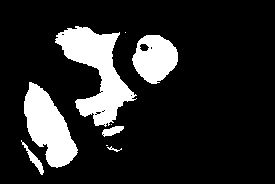
\includegraphics[width=\textwidth]{processed_data/orange_mask_0.jpg} 
      \caption{Máscara naranja de la imagen 1, autoría propia.}
      \label{fig:white_mask}
  \end{minipage}
  \hfill
  \begin{minipage}[t]{0.3\textwidth}
      \centering
      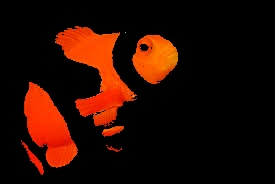
\includegraphics[width=\textwidth]{processed_data/orange_segmented_0.jpg}
      \caption{Segmentación naranja de la imagen 1, autoría propia.}
      \label{fig:white_segmented}
  \end{minipage}
  
\end{figure}

\begin{figure}[H]

  \begin{minipage}[t]{0.3\textwidth}
      \centering
      
\includegraphics[width=\textwidth]{processed_data/white_mask_0.jpg}
      \caption{Máscara blanco de la imagen 1, autoría propia.}
      \label{fig:orange_mask}
  \end{minipage}
  \hfill
  \begin{minipage}[t]{0.3\textwidth}
      \centering
      
\includegraphics[width=\textwidth]{processed_data/white_segmented_0.jpg}
      \caption{Segmentación blanco de la imagen 1, autoría propia.}
      \label{fig:orange_segmented}
  \end{minipage}
\end{figure}

\subsection{Segmentación multicolor}

\vspace{0.5cm}

El segmentado de múltiples colores se entiende como la creación de una máscara binaria por cada color de interés realizando posteriormente una superposición en 
una más genérica. Dado que las máscaras son binarias, basta con hacer una operación OR entre ellas para obtener la máscara que con la que filtrar las imágenes originales. 
Para ejemplificar este proceso, se han segmentado los colores naranja, blanco de la imagen 1, así como el blanco, rojo, verde, azul, amarillo y gris del logo de 
''Redbull King of the Air'' (el verde es el color por defecto del fondo de un png):

\vspace{0.5cm}

\begin{figure}[H]
  \centering
  \begin{minipage}[t]{0.3\textwidth}
      
\includegraphics[width=\textwidth]{processed_data/fish_mask_0.jpg} 
      \caption{Máscara multicolor de la imagen 1, autoría propia.}
      \label{fig:multicolor_mask}
  \end{minipage}
  \hfill
  \begin{minipage}[t]{0.3\textwidth}
      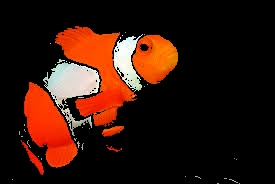
\includegraphics[width=\textwidth]{processed_data/fish_segmented_0.jpg}
      \caption{Segmentación multicolor de la imagen 1, autoría propia.}
      \label{fig:multicolor_segmented}
  \end{minipage}

\end{figure}

\begin{figure}[H]
  
  \begin{minipage}[t]{0.6\textwidth}
    
\includegraphics[width=0.3\textwidth]{data/king_of_the_air.png}
    \caption{Logo de ''Redbull King of the Air'',\\https://www.redbull.com/es-es/events/king-of-the-air.}
    \label{fig:redbull_original}
  \end{minipage}
  \hfill
  \hspace{1.5cm}
  \begin{minipage}[t]{0.6\textwidth}
    \includegraphics[width=0.3\textwidth]{processed_data/king_of_the_air_segmented.jpg}
    \caption{Segmentación multicolor\\del logo de''Redbull King of the Air'',\\ autoría propia.}
    \label{fig:redbull_segmentation}
  \end{minipage}

\end{figure}


\section{Filtro Gaussiano y Detección de bordes: Sobel y Canny}


\vspace{1cm}

El filtrado de imágenes es una técnica fundamental en el procesamiento de imágenes que permite mejorar la calidad de las imágenes, eliminar el ruido y resaltar 
características de interés. Habitualmente los

\section{Operadores morfológicos}

En esta sección, se implementan los operadores morfológicos de dilatación y erosión
utilizando un kernel de \(3 \times 3\) con valores de \(255\) (blanco) como structuring element. 

Se define el método de binarización, el cual convierte una imagen a escala de grises a una imagen 
binaria utilizando un umbral de \(127\). Este método emplea la función \textit{cv2.threshold} de 
OpenCV para realizar la conversión.

Se implementa el método de dilatación, que consiste en ampliar las áreas blancas de la imagen binaria. 
Para ello, se utiliza un padding de la imagen original para mantener las dimensiones tras el procesamiento. 
En este método, se recorren todos los píxeles de la imagen, y se reemplaza cada píxel por el valor máximo 
de sus vecinos en el kernel.

Asimismo, se implementa el método de erosión, que reduce las áreas blancas de la imagen. Al igual que en 
la dilatación, se utiliza un padding para conservar las dimensiones. En este caso, cada píxel se reemplaza 
por el valor mínimo de sus vecinos en el kernel.

% \begin{figure}[h!]
%   \centering
%   \begin{minipage}[b]{0.45\textwidth}
%       \centering
%       \includegraphics[width=\textwidth]{smorphological_operators/custom_dilate_0.png}
%       \caption{Ajuste fino de intersección de cuadrícula, autoría propia.}
%       \label{fig:izquierda1}
%   \end{minipage}
%   \hfill
%   \begin{minipage}[b]{0.45\textwidth}
%       \centering
%       \includegraphics[width=\textwidth]{src/morphological_operators/custom_erode_0.png}
%       \caption{Ajuste fino de intersección de cuadrícula, autoría propia.}
%       \label{fig:derecha1}
%   \end{minipage}

% \end{figure}

\end{document}



